\chapter{Functionalities required of historical language thesauri for research and education}
%\markboth{CHAPTER 2}{}


In order to improve the dissemination of historical language thesauri on the Web, not only is their content of importance but also the functionality required by their target audience. This chapter describes functionality required by users in academia, both for research and educational purposes, of editions of these lexicographic resources. In order to gather information on such functionality, a number of sources have been consulted. First, existing editions of historical language thesauri and handbooks on both thesauri and lexicography in general, which were also consulted in Chapter 1, provided valuable input. Second, academic reviews of these thesauri and notable research employing these resources offer further insights. Lastly, additional input has been collected from stakeholders -- experts in lexicography, linguistics and philology (amongst other fields) -- through dedicated stakeholder meetings, workshops, and feedback based on preliminary results in research and education in a research project titled `Exploring Early Medieval English Eloquence'.\footnote{The research project and its resulting case studies are discussed in Chapter 8. \hyperref[Appendix2.A]{Appendix 2.A} lists the functionality required by researchers participating in this project.} % largely overlaps with that found in other sources. %The chapter will therefore limit references to the research project to functionality not located in other, published sources. 
%The functionalities distilled through the three types of sources mentioned above is by no means exhaustive. Rather, as Chapter 8 will demonstrate, it enables the use of these lexicographic works in novel research and for introducing students to the lexis of a historical language and the nuances within its vocabulary. The resulting information on functionality is, therefore, a solid foundation for research, one to which further functionality may be added for more specific purposes. 
Within the remainder of this chapter, the present set of functionality gathered is detailed in five sections: navigation (\ref{sect:Stolk_thes-functionality:navigation}), resource views (\ref{sect:Stolk_thes-functionality:resource-views}), extension (\ref{sect:Stolk_thes-functionality:extension}), analyses (\ref{sect:Stolk_thes-functionality:analyses}), and data management (\ref{sect:Stolk_thes-functionality:data-management}).



\section{Navigation}
\label{sect:Stolk_thes-functionality:navigation}

\begin{comment}
\textcolor{red}{
R1. Navigation. A thesaurus can be approached in two manners: through its overarching taxonomy or through the lexis it organises (HTOED: ix). Both means are deemed key in allowing users -- both newcomers and frequent users -- to navigate the lexicographic content (Kay and Alexander, 2016: 368).
}
\end{comment}

The first and foremost functionality required of thesaurus editions is the ability for users to navigate their content. The preface to \textit{HTE} indicates that users have a choice in how to approach that content:
\begin{quotation}\noindent
There are two ways to approach a thesaurus: by familiarizing oneself with its structure and principles of organization, or, more commonly, by using its index to determine in which category or categories a word appears.\footnote{\textit{HTE1}, p. ix.}
\end{quotation}
Whether the one approach is truly used more commonly than another is less clear cut. Christian Kay, one of the editors of \textit{HTE}, mentions that the alphabetical index is there ``for convenience'' and may not be needed for ``confident and frequent users'' of the thesaurus.\footnote{Kay and Alexander, `Diachronic and Synchronic Thesauruses', p. 368.} Similarly, the editors of \textit{TOE} prompt the user to approach their thesaurus ``by subject rather than through the alphabetic index''.\footnote{\textit{TOE2}, p. xv.} Nevertheless, both means of navigation are offered to users of historical language thesauri and hence warrant further treatment.

\subsection{Navigation via the thesaurus structure}
Users can employ the topical structure of a thesaurus to move from meaning to lexical items conveying that meaning. In order to facilitate this approach, print editions of the historical language thesauri under discussion all include an outline of their topical system.\footnote{\textit{TOE2}, pp. v–viii; \textit{LSM}, pp. iv–xvii; \textit{HTE1}, pp. xxix–xxx; \textit{ShT}, pp. xvii–xxv; \textit{ScT}, pp. iv–vii.
\textit{DSSPIEL} has separated its outline over the table of contents for the primary categories (p. xix) and the sections that treat each of those categories. These sections begin with a list of the subcategories.} For those historical language thesauri that %employ a cumulative microstructure and as a result 
have three or fewer levels in their topical system, such as \textit{ScT}, this outline typically presents the system in its entirety. For those thesauri with a larger degree of specialization in their topical systems, termed distinctive thesauri by Christian Kay and Marc Alexander, the outline may be limited to the top categories in order to save space.\footnote{Kay and Alexander, `Diachronic and Synchronic Thesauruses', p. 370.} Such a limited outline is offered in the print editions of \textit{TOE} and \textit{HTE}, which contain over ten levels in their topical systems and provide an outline for the first two and three of these levels, respectively.
% NOTE: TOE4 has 11 levels; checked in TOE-LLD
%All other print editions of the historical language thesauri include a complete overview, although perhaps, in the case of \textit{DSSPIEL}, separated over the start of the sections that treat the primary categories rather than in the front matter.

Through the use of hyperlinks, electronic editions of historical language thesauri can supply users with the means to navigate the topical system in an interactive manner. The majority of the current electronic editions of these thesauri 
%\textit{HTE} found at the \textit{OED} website (\textit{HTE2}) 
offer an overview %of the topical system 
similar to those found in the print editions. The overviews of \textit{BTH}, \textit{TOE4}, \textit{HTE2}, and \textit{HTE3} are located on a single webpage, allowing the user to expand or collapse categories to show or hide subordinate ones. Only when selecting a specific category for viewing purposes will this edition show the senses contained within. Such a useful overview has not been offered by all Web-based editions of thesauri.  \textit{TOE3}, no longer available, and \textit{HTS} require the user to navigate the structure by taking single steps further down, or up, the hierarchy. A new webpage is loaded in the browser for each position in the topical system that the user passes through. In contrast, all electronic editions indicate the current position in the taxonomy through breadcrumbs, a trail of hyperlinks of the current category and ones superordinate to it. %Alongside navigation options to superordinate and to subordinate categories, these pages include the words and phrases located directly within the category currently viewed. The lack of a webpage that contains a complete overview of the topical system might be accounted for by the fact that the browsing system in place is perhaps thought to be more user-friendly. Both systems could, however, perfectly exist alongside each other.

%A larger problem with the browse system available is that all these electronic editions do not provide a page to start browsing from, one that lists all top categories. These top categories are referred to as the t1 categories. In order to view any of these categories, the user has to input its identification number via the Search menu. For the category ``Quiet, leisure, rest'', for instance, one has to input 18 as the t1 category number of interest in \textit{TOE4}. It is impossible for users, through these websites, to first view which main categories exist, what they are called, and what the identification numbers are associated with them. In effect, the approach of requiring users to choose for a category number before viewing which categories exist demands them to be familiar with the contents of the thesaurus before viewing it --- a flawed notion that results in an imperfect interface.

\subsection{Navigation via the thesaurus index}

The second manner in which users can approach a thesaurus is through an alphabetic index. Reviewers of historical language thesauri have called the availability of such an index ``necessary'' and even ``indispensable'' in order to find a word or phrase within the categories of thesauri.\footnote{Görlach, Review of \textit{TOE1}, p. 399; Momma, Review of \textit{TOE2}, p. 80.} The added value of an index seems to have been well understood by the editors of the historical language thesauri of Scots and English, since all their printed editions include an alphabetic index to their contents. 

Which parts of the contents are indexed alphabetically can vary between thesauri in print. The majority of the historical language thesauri treated here -- \textit{ShT}, \textit{LSM}, \textit{TOE}, and \textit{HTE} -- index their lexical senses (through their head-forms), but not their categories. The editors of the other two printed historical language thesauri have opted to base their index on English rather than their actual lexicon. As such, the index that complements \textit{DSSPIEL} is one to its categories, or headings, rather than to its categorized lexical items.\footnote{\textit{DSSPIEL}, p. 1505.} The index of \textit{ScT} is meant to provide ``a detailed signposting in English into the intricacies of Scots vocabulary'',\footnote{\textit{ScT}, p. xix.} listing near English equivalents to the Scottish senses, when available, as well as more generic English concepts taken from its English categories.\footnote{\textit{ScT}, p. xix.} In other words, this index incorporates elements from both the lexical senses (i.e., their definition) and the topical system in order to assist the reader, who is likely to learn more about Scots through the English language than through the Scots vocabulary directly.

Although they have their use for thesauri in printed from, alphabetic indexes are no longer essential for digital thesauri. Instead, the functionality required to find a word or phrase may be provided by a search system. Indeed, the digital editions of \textit{TOE} and \textit{HTE} sport such search systems and have abandoned an alphabetical index. These search systems offer a vast improvement over an index in three ways. The first is in terms of retrieval speed --- going back and forth between index and the thesaurus proper can now indeed take only ``a twinkling of an eye''.\footnote{Busse, `A Celebration of Words and Ideas', 
%: The Stylistic Potential of the \textit{Historical Thesaurus of the Oxford English Dictionary}', Review of \textit{HTE1} and \textit{HTE2}, \textit{Language and Literature} 21.1 (2012), 84–92
p. 804.} The second improvement is that both categories and lexical senses can be included in searches without any serious drawbacks in this method of access. Where textual editions were criticized for not containing alphabetical indexes to both categories and entries,\footnote{Görlach, Review of \textit{TOE1}, p. 399.} possibly due to limits on printing space imposed by publishers or to avoid too great a weight of the books for readers to handle them, the digital editions of \textit{TOE} and \textit{HTE} offer this sought-after ease of access through their new search systems. The third improvement offered by digital search systems is that lexical senses can now be located based on the additional information per sense, including the labels they carry. This allows searches to be restricted, for instance, to items of a particular part of speech or to those marked as `poetical'. Of course, it would be just as interesting to restrict searches to senses that do \textit{not} carry a given label, since these senses are implicitly marked by the editors as belonging outside of the group indicated by the absent label.\footnote{Svensén, \textit{A Handbook of Lexicography}, p. 315.} The possibility to exclude a label from searches would allow one, for example, to locate only non-poetical lexical senses. This functionality of exclusion of labels in searches is not yet provided by the current systems in place for the digital versions of \textit{TOE} and \textit{HTE}.%, and it is one that would surely benefit users of digital thesauri. %As the topic of filtering and querying will be discussed in section 2.2.4, I will not dwell on the subject any further presently.

\section{Resource views}
\label{sect:Stolk_thes-functionality:resource-views}

The second functionality required of thesaurus editions is the ability to view all the information available on a specific category or lexical item that a user chooses to inspect. For lexical items these resource views ideally contain the part of speech, language, and usage features; and for categories, their name and identification string.\footnote{See Chapter 1 for a thorough overview of information available in historical language thesauri.} Moreover, these overviews should indicate relations to other resources where relevant, such as, for categories, a list of the lexical senses that are allocated to the viewed location of the thesaurus taxonomy or, concerning lexical items, an overview of synonyms. % and the various branches of the taxonomy that contain one of the senses of the currently inspected word or phrase. 
These essential resource views are present in historical language thesauri (e.g., as entries in a printed thesaurus), albeit not always as complete as possible.

One piece of information useful for research, noted by both editors and reviewers of thesauri and absent from existing resource views of lexical items, is an overview of the different senses of a single lexeme.\footnote{See \textit{HTE1}, p. x; Ilson, `On the Historical Thesaurus of the Oxford English Dictionary', %Review of \textit{HTE1}, \textit{International Journal of Lexicography} 24.2 (2011), 241–60 (p. 256)
p. 256.} Such views of senses related through polysemy facilitate explorations of metaphorical and metonimical uses and offer a measure of ambiguity in utterances in which the lexeme in question occurs. Through these connections of individual lexemes, it is possible to detect which semantic fields in a language have close conceptual ties. For example, terminology surrounding sleep can be used metaphorically for death; temperature for emotions.\footnote{For both metaphorical ties mentioned, see \textit{Mapping Metaphor with the Historical Thesaurus}.} % (Glasgow, 2015). \url{http://mappingmetaphor.arts.gla.ac.uk}. Accessed October 31, 2016.
By mapping out metaphorical connections such as these, it is possible to gain a better understanding of the stylistic impact of metaphors and to grasp which groups of words are more easily used to symbolically represent other meanings.\footnote{Ibid.} Existing historical language thesauri of Scots and English, rather than including the information on senses related through polysemy in the resource view of a lexical item, rely on the user switching to either the index (in print editions) or the search engine (in digital editions) to obtain this knowledge on the lexical item inspected.

Resource views could also be employed to present details on elements other than categories and lexical items. Labels found in thesauri are valuable elements of information, too, that may warrant their own resource view. Such labels, which benefit from thorough descriptions, are utilized by researchers to investigate the usage features with which those labels are associated.\footnote{Brewer, `Labelling and Metalanguage', %in \textit{The Oxford Handbook of Lexicography}, ed. P. Durkin (Oxford, 2016), pp. 488–500 (p. 493)
p. 493; Norri, `Regional Labels in Some British and American Dictionaries'. %, \textit{International Journal of Lexicography} 9.1 (1996), 1–29.
See the discussion in section \ref{sect:Stolk_thes-content:diasystematic-labelling} of Chapter 1.} Providing resource views for these elements could assist researchers in finding helpful information on them, including a full name and description instead of only a code or abbreviation. Moreover, providing these resource views for labels can assist in retrieving the elements they mark. One such need is exemplified in Kathryn Allan's work on metaphor and metonymy, drawing on information from \textit{HTE}.\footnote{Allan, \textit{Metaphor and Metonymy}.} Lexical senses in \textit{HTE} were marked with labels that represent what Allan calls core concepts. Subsequently these custom labels were used to retrieve all items tagged with a specific core concept, such as ANIMAL or AGE.\footnote{Ibid., pp. 21–2.} Although the need for adding custom labels will be explored further in section \ref{sect:Stolk_thes-functionality:extension}, the demand for viewing a list of all items to which a label is applied can be satisfied through a resource view for this kind of element. Despite these reasons, none of the Web-based editions of historical language thesauri offer resource views for elements other than categories and lexical items. 


Lastly, resource views would benefit from the means to hide information deemed irrelevant to a user. This aspect has been noted by creators and reviewers of thesauri alike as important.\footnote{For an academic review discussing the possibility and desirability of creating subthesauri through such mechanisms of filtering, see Conner, Review of \textit{TOE1}, p. 888.} The editors of \textit{HTE}, for instance, state that the very purpose of their thesaurus is ``to provide a detailed record of the English vocabulary from the earliest times to the present, with sufficient accompanying information that, for any given period in the past, the user should be able to ascertain the exact state of the vocabulary (i.e., the `lexical system') which existed at that time''.\footnote{\textit{HTE1}, p. xiii.} They point out that the \textit{HTE} could thus be used to ``act as a thesaurus for any period in the past'', allowing one to determine which lexical items will have been available to Shakespeare.\footnote{\textit{HTE1}, p. xiv.} However, both digital editions of \textit{HTE} prevent the creation of a subthesaurus based on the recorded diachronic usage features, containing only those lexical senses that were available in Shakespeare's time --- or any other subthesaurus based on a set of criteria for that matter. Any sifting is left as manual labour to the user. \textit{TOE}, too, includes valuable tagging information, stating whether its items are found only in poetry or only in glosses, for example. Although \textit{TOE3} allowed viewing subthesauri based on the available tagging information, \textit{TOE4} no longer sports this helpful feature.\footnote{For a description of the previously available \textit{TOE} website and its feature to create subthesauri based on tagging information, see Stolk, `Welcoming the \textit{Thesaurus of Old English Statistics}', pp. 11–14.} In short, the existing digital versions of these thesauri lack the ability for their users to view only those items deemed of interest based on usage features and other information available --- a filtering ability applicable to both resource views and the mechanisms available to navigate a thesaurus.



\section{Extension}
\label{sect:Stolk_thes-functionality:extension}

The third functionality researchers require of thesaurus editions is the ability to extend them, connecting additional information to their content in order to enrich or reuse that existing data. Examples of such extensions are indications of date and dialect, results from corpus searches, and indications whether a word or meaning is found in a particular text, context, or is notable in some other qualitative or quantitative way. The functionality to extend thesaurus content offers users the means to have the thesaurus reflect their own interests and to share salient information with others. This section discusses two forms of extension: 1) elaboration on thesaurus content and 2) connecting other bodies of knowledge to a thesaurus.

\subsection{Elaboration on content}

Many scholars desire labelling information in historical language thesauri beyond what has been made available and, for that purpose, the ability to elaborate on thesaurus content. In a review of \textit{ShT}, for instance, Christian Kay expresses that she finds it ``frustrating that nothing other than the part of speech of each word is offered to the user''.\footnote{Kay, Review of \textit{ShT}, p. 72.} A second example is the existing tagging information per lexical item in \textit{TOE}, which is deemed helpful and efficient,\footnote{Cavill, `Names and Things in Anglo-Saxon and Early Norman England', %Review of \textit{TOE1} and \textit{Words, Names and History: Selected Writings of Cecily Clark} ed. by Peter Jackson, \textit{Nottingham Medieval Studies} 41 (1997), 186–91 (p. 186)
p. 186; Conner, Review of \textit{TOE1}, %\textit{Speculum} 73.3 (1998), 887–9 (p. 888)
p. 888.} but also thought to be rather limited.\footnote{Bremmer, `Treasure Digging in the Old English Lexicon', %Review of \textit{TOE2}, \textit{NOWELE} 40 (2002), 109–14 (p. 111)
p. 111; Görlach, Review of \textit{TOE1}, p. 399; Dance, Review of \textit{TOE1}, p. 313.} Indications of date and dialect, for example, are notably absent. 
%A case in point of information notably absent in \textit{TOE} is indications of date and dialect for its lexis. 
As it stands, all items are treated as belonging to ``a single geographically and temporally indistinguishable mass''.\footnote{Dance, Review of \textit{TOE1}, p. 313.} 
Researchers certainly possess further insights on these topics: Rolf H. Bremmer Jr asserts that the dialectal origins of many Old English words can be pinpointed globally as Anglian, West-Saxon, or Kentish and that such information would be worthwhile to add to \textit{TOE}.\footnote{Bremmer, `Treasure Digging in the Old English Lexicon', pp. 111–12.} The added knowledge would facilitate research into the impact of regional influences on the Old English vocabulary as it has come down to us and, further along the line, on present-day English. Researchers participating in the workshop series, too, indicated the usefulness of adopting custom labels to add further distinctions in genre, dialect, diachronic usage, and etymology.\footnote{See Chapter 8 and \hyperref[Appendix2.A]{Appendix 2.A.}}


The means to elaborate is also desired on elements other than labels for lexical senses. Kathryn Allan, for example, points out that sections of \textit{HTE} available to her lacked lexical items that she thought belonged in these locations and, consequentially, wished to insert there.\footnote{Allan, \textit{Metaphor and Metonymy}, p. 20.} Similarly, certain lexical items may warrant marking to be stricken from a thesaurus --- especially if dealing with words that appear to lack evidence for their existence, so-called ghost words.\footnote{Hartmann and James, \textit{Dictionary of Lexicography}, s.v. `ghost word'.}  %Allan's desire, then, has been to reuse an existing topical system and most -- but not all -- of its categorized lexical senses.
%The means to expand the topical system has been noted as a desirable feature, too. 
Another case for elaborating has been made by Nils Århammar, who suggests supplementing \textit{DSSPIEL} with lexical items of various stages of the Frisian language.\footnote{Århammar, `A Frisian Supplement to Buck's Dictionary of Indo-European Synonyms?'.} Additions and refinements to the topical system, too, are valued for research purposes. Christian Kay, in her review on \textit{ShT}, professes that she would welcome a further subdivision in its existing system of rather abstract categories. Such a fine-grained division ``would make it easier to identify areas of high lexicalisation [i.e., where elaboration of vocabulary is notable], and, with the help of other reference works, to examine areas where Shakespearean innovations are prevalent''.\footnote{Kay, Review of \textit{ShT}, p. 73.} %In effect, this process would change the character of the thesaurus from cumulative to distinctive.

A perhaps more drastic fashion in which to extend thesaurus content is by creating a new topical system to supplant the existing one, reusing and extending only lexical items recorded in a thesaurus. A case in point is Thijs Porck's study of the conceptualisation of old age in early medieval England, which draws on the contents of \textit{TOE}, but replaces the existing categorisation with one more suitable to capture nuances newly established in the semantic field under investigation. Lexical senses from four separate \textit{TOE} categories are grouped together as all belonging to the category of ``Human old age''.\footnote{Porck, `Growing Old among the Anglo-Saxons', pp. 68–9.} The new categorisation system fashioned for these items %is presented visually by means of a diagram.\footnote{T. Porck, `Growing Old among the Anglo-Saxons: The Cultural Conceptualisation of Old Age in Early Medieval England' (unpublished D.Phil. dissertation, Leiden University, 2016), p. 71.} The main category of \textit{Old age} is subdivided into
contains semantic domains, such as ``Positive development'', ``Wisdom'', and ``Authority''. Similarly, \textit{BTH} indicates that it reuses categories from the topical system of \textit{HTE}, ``though these were occasionally modified in order to capture the ways in which conceptions in the Middle Ages differed from those of the present day'', and adds words from Anglo French, spoken in England alongside Middle English after the Norman Conquest in 1066.\footnote{See \textit{BTH}, section `About'.} In short, many scholars wish to extend the content of historical language thesauri, to varying degrees, for research purposes.


% "The vocabulary in the Bilingual Thesaurus comes from the Anglo-Norman Dictionary, the Middle English Dictionary and the Oxford English Dictionary. Its structure makes use of the category structures of the Historical Thesaurus though these were occasionally modified in order to capture the ways in which conceptions in the Middle Ages differed from those of the present day." @ https://thesaurus.ac.uk/bth/about/


Unfortunately, any elaboration on thesauri content and subsequent sharing of these additions is currently not facilitated by most of the published forms of the historical language thesauri treated here. Only \textit{HTS}, one of the thesauri available online, sports a comment section in which users can share their thoughts publicly (see Figure \ref{fig:Stolk_thes-functionality:HTS-annotations}). All other publications of the thesauri analysed do not provide the means for additions to be made by anyone other than their editors. One can scribble additions in the margins of paper copies or refer to bits of information via a textual reference, but these acts do not extend the conceptual thesaurus: The additions either affect only a single copy (in the case of annotations in the margins) or are stored in a different location and format that hampers simultaneous and integrated access to the content of both the original and its additions.

%The ability for users to contribute their own thoughts to thesaurus content is, for the historical language thesauri analysed, solely made available in \textit{HTS}. This online thesaurus sports a comment section in which users can share their thoughts publicly (see Figure \ref{fig:Stolk_thes-functionality:HTS-annotations}). Solutions beyond a database hosted by the publisher of the lexicographic work can be found on the Web, too. The \textit{Merriam-Webster} dictionary, for instance, incorporates functionality from Facebook for capturing, storing, and viewing user comments per dictionary entry. These comments are, like those at \textit{HTS}, moderated by the publishers of the lexicographic work. User comments and annotations can also be stored beyond the moderating abilities of publishers, though, as is the case with the tool Hypothesis. This online tool can serve as portal through which users can view webpages (including those of online lexicographic resources), highlight text, and save their tags and comments publicly or privately in the Hypothesis database. These solutions share a disadvantage: They forestall running automated analyses over the original content and thesaurus data in unison, which is functionality desired by researchers (see section \ref{sect:Stolk_thes-functionality:analyses}).

\begin{figure}[htb]
    \centering
	\framebox[\textwidth]{
		\scalebox{0.7}[0.7]{
			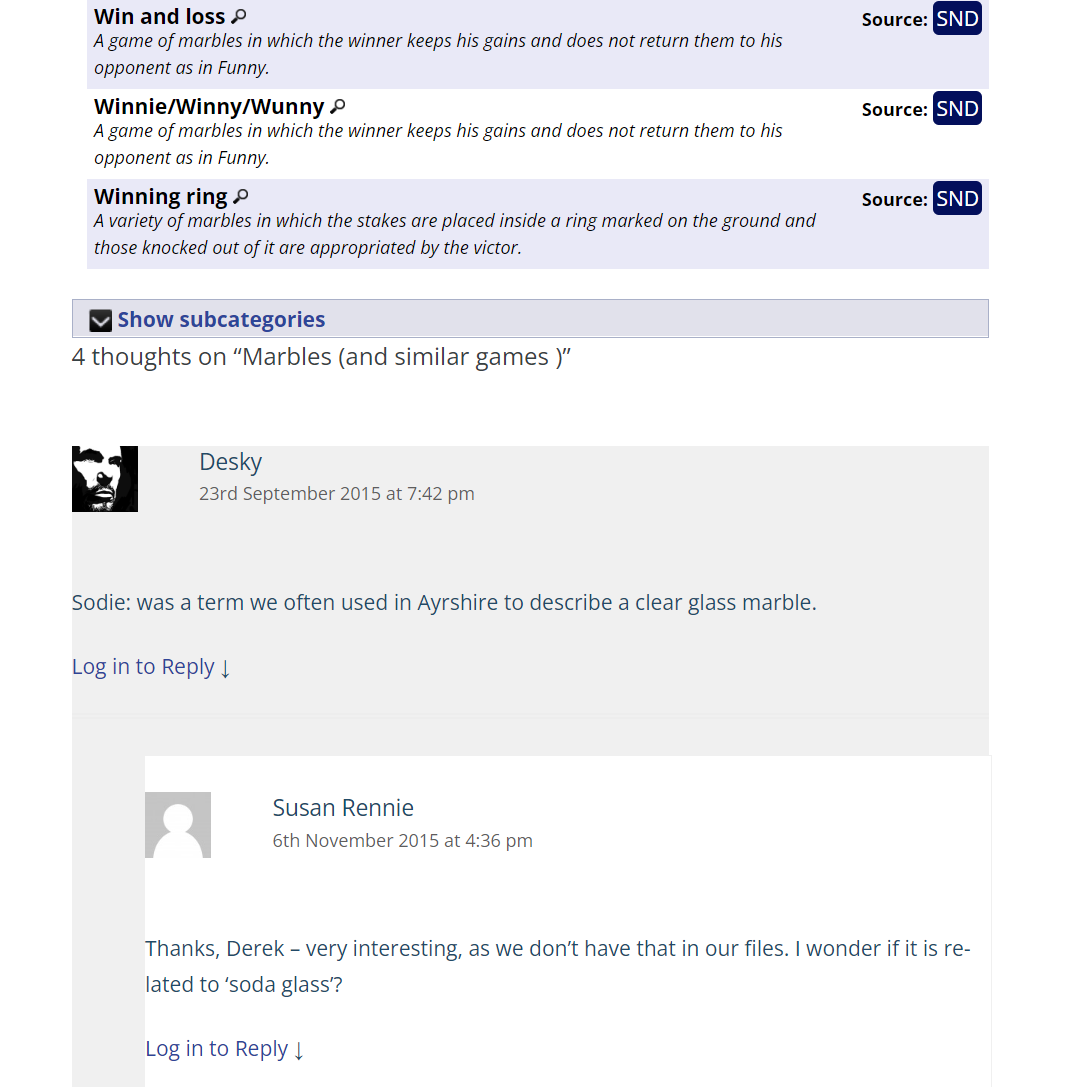
\includegraphics{Stolk_thes-functionality/fig/HTS-annotations.png}
		}
	}
	\caption[]{\label{fig:Stolk_thes-functionality:HTS-annotations} Comments by users on \textit{HTS} category  ``%03.13.01.05.02.14.03 n 
	Marbles (and similar games )''.}
\end{figure} 


\subsection{Connecting bodies of knowledge}% to thesaurus content}

Expansion can come not only in the form of elaboration on existing thesaurus content, but also by connecting other bodies of knowledge to a thesaurus. The desire for such functionality is expressed both by scholars who utilise or review the thesaurus and the editors themselves. The introduction to the paper editions of \textit{TOE}, for instance, states the following: ``Should a precise meaning be wanted, a dictionary is needed''.\footnote{\textit{TOE2}, p. xv.} \textit{ScT} contains a similar statement, referring readers to the \textit{Concise Scots Dictionary} for etymology and pronunciation of items from its lexis.\footnote{\textit{ScT}, p. xv.} The introduction to \textit{HTE}, too, indicates that connectivity between the thesaurus and a dictionary with supplementing information, the \textit{Oxford English Dictionary}, is desirable.\footnote{\textit{HTE1}, p. xiv.} That such relations between bodies are worth exploring is not only suggested by editors but also taken to heart by users. David Crystal, for one, in his explorations of \textit{HTE} content has also turned to related definitions and citations from the \textit{OED}.\footnote{Crystal, \textit{Words in Time and Place}, %: Exploring Language through} The Historical Thesaurus of the Oxford English Dictionary (Oxford, 2014), 
p. xv.} Likewise, Kathryn Allan has performed analyses of \textit{HTE} items ``by looking closely at etymological information supplied in the \textit{OED}''.\footnote{Allan, \textit{Metaphor and Metonymy}, %: A Diachronic Approach}, Publications of the Philological Society 42 (Malden, 2008), 
p. 21.} Relations between bodies of knowledge like the aforementioned ones can, as the editor of \textit{ScT} points out, act as ``a series of step-by-step doorways into the heart of a national culture''.\footnote{\textit{ScT}, p. ix.}

Relating bodies of knowledge to each other can be achieved in a number of ways. The extent to which the user is facilitated in retrieving and combining information from multiple bodies varies per solution. The most basic level of relating two bodies is by mentioning to users that such a relation exists, possibly in the introduction. This method is applied in many print editions of historical language thesauri.\footnote{See Chapter 1, section \ref{sect:Stolk_thes-content:ExternalReference}.} It is wholly left to the user to access the second body of knowledge and subsequently to locate the desired complementary information. A more user-friendly solution of relating two bodies is by making an explicit mention of where exactly such complementary information can be found. External references per lexical sense do just that.

Although an external reference at a lexical sense directs users to the appropriate location in another body, paper editions still require users to move from body to body in order to accumulate the information sought after. Facilitating users in the fullest manner possible comes from connectivity in a digital environment, such as through hyperlinks. In fact, true connectivity would allow users to access and query knowledge from multiple bodies at the same time, without having to manually move from the one to the other. Unfortunately, as McCracken notes, connecting bodies is ``curiously underexplored in lexicography'', even though it is ``a familiar topic in the context of knowledge bases''.\footnote{McCracken, `The Exploitation of Dictionary Data and Metadata', %in \textit{The Oxford Handbook of Lexicography}, ed. P. Durkin (Oxford, 2016), pp. 501–14 (p. 513)
p. 513.} By applying conventions found in the context of knowledge bases, it should therefore be possible to remove the somewhat isolated status of historical language thesauri. For users to have complementary information at their fingertips, editors and publishers of thesauri may well want to shift their focus from ``aspirations of completeness and comprehensiveness'' to ``connectivity and interoperability''.\footnote{Ibid., p. 513.}
%J. McCracken, `The Exploitation of Dictionary Data and Metadata', in \textit{The Oxford Handbook of Lexicography}, ed. P. Durkin (Oxford, 2016), pp. 501–14 (p. 513).



\section{Analyses}
\label{sect:Stolk_thes-functionality:analyses}

The means to perform statistical analyses is another key feature sought after by researchers.\footnote{Evidenced by \hyperref[Appendix2.A]{Appendix 2.A}, which indicates such functionality has been required by researchers in the project `Exploring Early Medieval English Eloquence'.} Such analyses, utilizing the onomasiological structure of the thesaurus and features of the lexis it contains, facilitate investigations into a range of aspects encoded in the lexicon: cultural elaboration, semantic domains and their cultural connotations, stylistic preferences of authors, use and development of metaphors, and so on.\footnote{See, for instance, \textit{ShT}; Crystal, \textit{Words in Time and Place}; \textit{Mapping English Metaphor Through Time}; Porck, `Growing Old among the Anglo-Saxons', pp. 59–71; Diller, `Measuring the Growth of Semantic Fields'.} Regrettably, few editions of historical language thesauri offer functionality for even the most rudimentary of analyses.

\textit{ShT}, Christian Kay observes, sorely lacks a simple count of lexical items under a category.\footnote{Kay, Review of \textit{ShT}, p. 73.} Such counts indicate the degree of lexicalization, also known as cultural elaboration, of semantic concepts.\footnote{Wierzbicka, \textit{Understanding Cultures through Their Key Words}, pp. 10-11.} The underlying hypothesis for the importance of these figures is that domains that are important in a culture are heavily encoded in the language of that community, providing its speakers with a multitude of nuances to discuss the subject. For thesaurus content in a digital environment, this statistic is relatively straightforward to obtain. Even so, many thesauri -- both paper and electronic editions -- do not include these statistics in their editions, including the paper editions of \textit{TOE} and \textit{HTE}. However, their electronic editions \textit{TOE3}, \textit{TOE4}, and \textit{HTE3} currently indicate the number of lexical senses located at any given category but, regrettably, without presenting the accumulated figure for that category and its subordinate categories, i.e., for the semantic domain.\footnote{In June 2017, \textit{HTE3} was updated to include the means to generate heatmaps and sparklines, visualizations that indicate degrees of lexicalization throughout the recorded history of the English language.} The larger the semantic domains analysed, the more valuable it will be for researchers to have these statistics automatically generated as opposed to calculating them manually. In \textit{TOE}, for instance, 1,348 lexical senses evoke the concept ``13.02 War'', whereas the nine co-ordinate domains for peace encompass a mere 119 lexical senses.\footnote{The nine co-ordinate categories for peace are the category ``13.01 Peace, state of law and order'' and the subcategories ``13|01 Peace, absence of dissension'', ``13|02 Unanimity, concord, agreement'', ``13|03 n. Good terms, rapport'', ``13|04 Peace, freedom from hate'', ``13|05 Peace among dwellings'', ``13|06 Accordant, not at variance'', ``13|07 Peacefully, peaceably'', and ``13|08 To agree, settle''.}

Statistics more nuanced than a count of all items located at a specific category are absent from all editions of historical language thesauri. This absence hampers researchers in utilizing the semantic information encoded by the topical system for an onomasiological analysis of lexical items with specific characteristics. Salient information on lexis -- such as period, region, register, or use by a specific author -- can form the basis of investigations into their spread across the semantic hierarchy, be it horizontally over the various semantic fields or vertically between levels of specificity in meaning attributed to the lexical items selected. Thus, the hierarchy of a historical language thesaurus has the potential to act as ``summary of the semantic framework'' and yield onomasiological profiles for those words and phrases in which researchers are interested.\footnote{Kay, `Food as a Fruitful Source of Metaphor', p. 77.} Additionally, researchers participating in the workshop series indicated the desire to contrast analyses between different languages and other features attributed to lexical items.\footnote{See \hyperref[Appendix2.A]{Appendix 2.A}.}

% "I have also suggested that levels of metaphor might be examined in terms of the HTOED hierarchy. Gentner and Bowdle point out that novel metaphors tend not to have meaning in isolation but become meaningful when associated with a target (2008: 115-16). HTOED hierarchies can supply a summary of the semantic framework in which both source and target terms occur, pinpointing the category and the taxonomic level within the category. In the case of polysemous terms, category membership can also help to identify likely links." (C. Kay, p.77 of chapter in book Mapping Metaphor)

%A thesaurus, Patrick Conner argues in his review of \textit{TOE}, ``offers information that its compilers may never have had in mind'' -- information that may well be worth looking into further.\footnote{Conner, Review of \textit{TOE1}, p. 889.} 

%An example of a welcome statistic of thesaurus content 
%(a query that the digital versions of \textit{TOE} and the stand-alone version of \textit{HTE} currently do not allow) 
%would be to provide statistics 
%is on the sizes of the semantic fields captured by its topical system. As Wierzbicka notes, important concepts in a society often witness cultural elaboration, that is, the availability of a relatively large number of words to express related notions and the nuances between them.\footnote{See A. Wierzbicka, \textit{Understanding Cultures through Their Key Words: English, Russian, Polish, German, and Japanese}, Oxford Studies in Anthropological Linguistics 8 (New York, 1997), pp. 10–11.} Supplying users with such key information on statistics is straightforward within a digital environment, without them having to count the lexemes or relevant senses manually.%\footnote{I have demonstrated that this is indeed possible in previous research. See Stolk, `Welcoming the \textit{Thesaurus of Old English Statistics}'.} 
%By way of illustration, the vocabulary for \textit{bondage, slavery} is quite sizeable in \textit{TOE}, ``show[ing] how this warrior society [i.e., that of the Anglo-Saxons] was sustained by a class of unfree [...] men and women''.\footnote{Momma, Review of \textit{TOE2}, p. 80.} Another striking example is that \textit{TOE} lists thirty-six Old English words for cloak-like garments. The great variety in words available to the Anglo-Saxons to describe these garments ``suggests that cloaks were a common garment, worn by different social classes''.\footnote{\textit{Learning with the Online} Thesaurus of Old English, eds. C. Hough and C. Kay (Glasgow, 2007). \url{http://oldenglishteaching.arts.gla.ac.uk}. The quotation is taken from the section `Unit 5 Clothing'. Accessed on October 31, 2016.} 


%Thesauri are valuable in analysing the vocabulary of a language community. Scholars have made use of these lexicographic works to investigate a range of aspects encoded in the lexicon: cultural elaboration, semantic domains and their cultural connotations, stylistic preferences of authors or in certain texts, and the use and development of metaphors (e.g., Spevack, 1993; Crystal, 2014; Anderson, Bramwell, and Hough, 2016; Porck, 2016: 59–71, 239–294; Diller, 2017).20 Functionality to perform such analyses is therefore valued greatly for research based on thesaurus content. A key requirement for Evoke in opening up thesauri, then, has been to allow users to perform statistical analyses (cf. R4). The analyses should work on the original thesaurus content but, with the ability of users to extend the thesaurus with their own information, also on additional content created by users. This section treats two manners in which users of the Evoke interface can perform analyses: (1) viewing default analyses and (2) building custom queries.21






\section{Data management}
\label{sect:Stolk_thes-functionality:data-management}

The fifth functionality required for research is the ability to manage the data under investigation, a demand that is largely the consequence of the need to extend thesaurus content.\footnote{This functionality has been requested and used by researchers in the project `Exploring Early Medieval English Eloquence' (see \hyperref[Appendix2.A]{Appendix 2.A}). For the need to extend thesaurus content, see section \ref{sect:Stolk_thes-functionality:extension}.} An important component of data management, necessary to support the extension of data by researchers, concerns personal additions, such as annotations and labelling. Researchers who supplement a historical language thesaurus with such additional knowledge should retain full control over their own data, including the ability to display or hide their annotations, create backups of their additions, and share their data with others.


A second component of data management, applicable to historical language thesauri extended by other data sources, is the means to select which of these sources are deemed relevant for researchers' explorations.\footnote{This functionality has been requested and used by researchers in the project `Exploring Early Medieval English Eloquence' (see \hyperref[Appendix2.A]{Appendix 2.A}).} Web-based editions of thesauri should allow for sets of information to be combined, based on the user's selection, for viewing and analyses, thus supporting researchers in their onomasiological explorations of lexis and any salient features captured. An advanced form of this functionality ought to support choosing for a certain revision of a data source, too, in cases where multiple are available. Revisions of digital historical language thesauri are certainly not shunned by their editors.

At its initial publication, the first digital edition of \textit{TOE} contained some corrections to its printed counterpart. These included changes of usage information and additions of new words, on the basis of new knowledge, which stemmed ``largely from completed sections of the Toronto Dictionary of Old English''.\footnote{Kay, `\textit{A Thesaurus of Old English} Online', pp. 36–40.} The exact alterations were left unspecified, though these will have mostly concerned lexical items starting with the letter F: between the publication of the second impression in print in 2000 and the first publication of the electronic edition in 2005, the Toronto dictionary only published its findings on Old English words starting with that letter.\footnote{The section on the letter F was published in 2004. See the `Publications' section of \textit{DOE}. Accessed on October 31, 2016.} As for any further updates to electronic editions, Kay mentioned that the taxonomy ``will, of course, be subject to rolling revision'' as the electronic environment allows for such changes.\footnote{Kay, `\textit{A Thesaurus of Old English} Online'.} Indeed, the number of items the online \textit{TOE} contains has increased from the 50,706 items Kay mentions in her article for the initial release of the electronic edition to 51,483 items on 26 May 2017.\footnote{An export of the \textit{TOE} database as it was on 26 May 2017 has kindly been provided to the author by the University of Glasgow.} %Revisions in the digital edition, then, are certainly not shunned -- a practice not limited to \textit{TOE} but also found with other thesauri, including \textit{HTE}.\footnote{See section `Versions of the \textit{Thesaurus}' of \textit{HTE3}. Accessed on October 31, 2016.}

When digital thesauri are subject to ongoing revisions, it may present difficulties for scholars to work with them.\footnote{See also Allan's remark on working with information from \textit{HTE}: ``It seemed preferable, and more theoretically justifiable, to work with the data as it existed at a particular stage of \textit{HTE}, whilst acknowledging that this may be incomplete. This is especially the case given the current revision of the \textit{OED}, which will in turn affect \textit{HTE} data and may lead to a number of insertions and changes in later editions'' (\textit{Metaphor and Metonymy}, p. 20).} Firstly, it could mean that the contents change whilst the scholar is doing research that involves the contents of the thesaurus. A lexical item could no longer be included under the category it used to be present in, and a category might have moved within the topical system. In effect, such changes during research entails scholars work with material that is ever in progress and for which it becomes difficult to discuss that reference body as a whole or even partially. Secondly, such revisions can make it more difficult to ensure verifiability of performed research. One of the important reasons why articles include references to the material they employed is that this practice allows others to review their work, verify whether the source material is accurate and reliable, and that the results are justifiable and could be reproduced if so desired.\footnote{See, for instance, the common ethics and responsibilities within science regarding the treatment of data and the sharing of research results as discussed in Gauch Jr, \textit{Scientific Method in Brief}, pp. 226–30.} With a reference body that is unstable, references to its contents may not provide the verifiability desired. Note that for publications in print, no such difficulties are present. Scholars can select an edition available at the moment of writing, employ that particular edition consistently, and have their references include the information on which edition should be consulted for purposes of verification.

In order to ensure that scholars can choose a particular edition or revision of a historical language thesaurus, the publication environment will need to support a form of versioning. That is to say, the thesaurus should be accessible under a system that allows users to view the taxonomy in each of its stages, enabling scholars to view and refer to the taxonomy in the state it was for a certain publication that made use thereof. Some digital reference bodies already provide such means to look into earlier states. Entries of the third edition of the \textit{OED}, for instance, contain links to the corresponding entries from the previous edition.\footnote{See \textit{OED Online}.} Maintaining separate editions online, similar to how this is the case for publications in print, will also open the possibility to pinpoint which changes have been made from one revision to the next, where they are located in the topical system, and possibly even for what reasons these have been made. Such information could help scholars in determining how up-to-date the taxonomy is, and whether they agree with the adjustments made, rather than having to analyse such matters themselves. Presently, such functionality is missing from all historical language thesauri in an electronic form treated here.



\section{Conclusion}

Drawing on existing historical language thesaurus editions, academic reviews, and research employing these resources, the current chapter has addressed functionality desired by researchers. An overview of the five functionalities that have been discussed is presented in Table \ref{table:Stolk_thes-functionality:requirements}. 
%
\begin{table}[h!]
    \centering
    \small
    \begin{tabular}{llp{8.25cm}}
    \toprule
        \textbf{Code} & \textbf{Name} &
        \textbf{Description} \\ 
    \midrule
    R1 & Navigation & 
    Approaching a thesaurus should be possible in two manners: through its overarching taxonomy or through the lexis it organises. \\
    R2 & Resource views & 
    Complete overviews of available information are to be presented on any given resource within a thesaurus that a user chooses to inspect. \\
    R3 & Extension & 
    Thesaurus content should be extendable, allowing users to connect additional information to existing content. \\
    R4 & Analyses & 
    Statistical analyses, utilizing the onomasiological structure of the thesaurus and features of the lexis it contains, should be made possible. \\
    R5 & Data management & Users must have full control over their own data and the ability to select which data sources are deemed relevant for their explorations, allowing sets of information to be combined for viewing and analysis. \\
%    R6 & Versioning & \textcolor{red}{x} \\
    \midrule
    \end{tabular}
    \caption[]{\label{table:Stolk_thes-functionality:requirements}Functionality required by researchers of historical language thesauri.}
\end{table}
%
%\noindent
Inclusion of this functionality varies in the existing editions of the historical language thesauri analysed. Whereas all editions offer navigation (through the topical system and through an index) and resource views, the ability to extend their content is found in only one thesaurus (i.e., \textit{HTS}) and is limited to sharing user comments. The effect of this lack of options to extend these thesauri is that, unsurprisingly, the need and mechanisms for data management are in these cases absent, too. Similarly, analysing thesaurus content through automated means is, across all thesauri, either minimal or vastly underexplored when considering the additional information that the semantic frameworks formed by these lexicographic works have the potential to yield. In short, the functionality identified here as required for research and education -- navigation, resource views, extension, analyses, data management -- should open new research avenues when incorporated into the dissemination of historical language thesauri. Sharing this set of functionality with researchers will greatly facilitate exploring the lexis of a historical language through a semantic lens.


% Chapter 2 addresses research sub question 2: ``What are the main features, or functionality, of historical language thesauri that are desired for research?'' This chapter consults, in addition to the very same sources for Chapter 1, academic reviews of these thesauri and notable research employing them. These sources help establish which aspects of the existing historical language thesauri are deemed an asset, and which were found wanting or absent. Further input was gathered through a series of workshops surrounding a single thesaurus (TOE) in order to obtain further research needs. The resulting information on desired functionality -- i.e., browsing, expansion, querying, and reuse -- has been translated to a set of requirements for the digital form proposed for thesaurus publications on the Web and for the web application developed for interacting with these lexicographic resources.




\begin{comment}
In order to facilitate research into thesauri, the first step in making Evoke was to gauge the research needs that it could answer. On the basis of published reviews of thesauri as well as a number of research cases, five requirements were established that the new web application had to meet. The first three requirements (R1–R3) were gathered for the first version of Evoke. The remaining two requirements (R4–R5) were formulated for subsequent iterations of the application and were collected from stakeholders -- experts in lexicography, linguistics and philology (amongst other fields) -- to ensure that the software is intuitive and useful for both research and educational purposes. Stakeholder requirements were gathered by several means: dedicated stakeholder meetings, workshops, and feedback based on preliminary results in research and education projects. Additionally, requirements on the architecture (AR1–AR3) were based on best practices for data on the Web, transparent data management, and limitations imposed by licensing schemes of existing lexicographic resources.

R1. Navigation. A thesaurus can be approached in two manners: through its overarching taxonomy or through the lexis it organises (HTOED: ix). Both means are deemed key in allowing users -- both newcomers and frequent users -- to navigate the lexicographic content (Kay and Alexander, 2016: 368 %Kay, C. and M. Alexander, `Diachronic and Synchronic Thesauruses').

R2. Resource views. Complete overviews of available information are to be presented on any given resource within a thesaurus that a user chooses to inspect. These overviews must indicate relations to other resources where relevant, such as listing the words that are allocated to the viewed location of the thesaurus taxonomy, or indicating the various branches of the taxonomy that contain one of the senses of the currently inspected word or phrase.

R3. Extension. The application should allow users to extend a thesaurus, connecting additional information to its content (cf. Bremmer Jr, 2002: 111; Görlach, 1998: 399; Dance, 1997: 313; Kay, 1996: 72). Examples of such extensions are indications of date and dialect, results from corpus searches, and indications whether a word or meaning is found in a particular text, context, or is notable in some other qualitative or quantitative way. This functionality offers users the means to have the thesaurus reflect their own interests and to share salient information with others.

R4. Analyses. Thesauri are valuable for investigations into a range of aspects encoded in the lexicon: cultural elaboration, semantic domains and their cultural connotations, stylistic preferences of authors, use and development of metaphors, and so on (e.g., Spevack, 1993; Crystal, 2014; Anderson, Bramwell, and Hough, 2016; Porck, 2016: 59–71, 239–294; Diller, 2017). Statistical analyses, utilizing the onomasiological structure of the thesaurus and features of the lexis it contains, are therefore a key functionality.

R5. Data management. Proper data management should be an essential aspect of the application in facilitating onomasiological research. Users must have full control over their own data (e.g., creating backups, sharing their data with others) and the ability to select which data sources are deemed relevant for their explorations, allowing sets of information to be combined for viewing and analysis.

AR1. Interoperable data form. The software is to read and display resources published as Linguistic Linked Data. This vocabulary, and the underlying data format (RDF), facilitate reuse and interoperability of linguistic resources according to the FAIR data principles (Wilkinson et al., 2016; Lóscio et al., 2017).

AR2. Decentralized data. The software must be capable of accessing data stored in a decentralized manner rather than relying on a central database, thereby stimulating a separation of data storage and services. Such separation is intended to remove barriers in selecting alternative solutions on both fronts, i.e., where the data is hosted and which application suits the needs of the user best (Verborgh, Wrigley, and Ballardini, 2019).

AR3. Support limited licenses. It is not uncommon to find lexicographic resources subject to licenses meant for viewing only, stipulating that users are not allowed to copy or download a substantial portion of the entire resource.9 A Thesaurus of Old English is one such work. The architecture of the application must allow interacting with and extending resources that are available under a license limiting access to browsing, in addition to those available under fully open access.

\end{comment}



\section*{References}

\begin{list}{}%
{\leftmargin=0.5in \itemindent=-0.5in}
\setlength{\itemsep}{0pt}
\setlength{\parskip}{0pt}
\setlength{\parsep}{0pt}


%%%%%%%%%%%%% 

%\item 
%Adamska-Sałaciak, A., Review of \textit{HTE1}, \textit{International Journal of Lexicography} 23.2 (2010), 227–33.

\item %CITED IN CHAPTER
Allan, K., \textit{Metaphor and Metonymy: A Diachronic Approach}, Publications of the Philological Society 42 (Oxford, 2008).

\item % CITED IN CHAPTER
Århammar, N., `A Frisian Supplement to Buck's Dictionary of Indo-European Synonyms?', \textit{Us Wurk} 21-22 (1972-1973), 241-5.

\item % CITED IN CHAPTER
Atkins, B. T. S. and M. Rundell, \textit{The Oxford Guide to Practical Lexicography} (Oxford, 2008).

\item %CITED IN CHAPTER
Bremmer Jr, R. H., `Treasure Digging in the Old English Lexicon', Review of \textit{TOE2}, \textit{NOWELE} 40 (2002), 109–14.

%\item %
%Brewer, C., `Authority and Personality in the \textit{Oxford English Dictionary}', \textit{Transactions of the Philological Society} 103.3 (2005), 261–301.

%\item %
%Brewer, C., `Prescriptivism and Descriptivism in the First, Second and Third Editions of \textit{OED}', \textit{English Today} 26.2 (2010), 24–33.

%\item 
%Brewer, C., Review of \textit{HTE1}, \textit{The Review of English Studies} 61.252 (2010), 801–5.

\item % CITED IN CHAPTER
Brewer, C., `Labelling and Metalanguage', in \textit{The Oxford Handbook of Lexicography}, ed. P. Durkin (Oxford, 2016), pp. 488–500.

\item % CITED IN CHAPTER
\textit{BTH} = \textit{The Bilingual Thesaurus of Everyday Life in Medieval England}, eds. (Glasgow, 2019). \url{https://thesaurus.ac.uk/bth/}. Accessed: 15 March 2022.

%\item %
%Buck, C. D., \textit{A Dictionary of Selected Synonyms of the Principal Indo-European Languages: A Contribution to the History of Ideas} (Chicago, 1949).

\item %% CITED IN CHAPTER
Busse, B., `A Celebration of Words and Ideas: The Stylistic Potential of the \textit{Historical Thesaurus of the Oxford English Dictionary}', Review of \textit{HTE1} and \textit{HTE2}, \textit{Language and Literature} 21.1 (2012), 84–92.

\item %% CITED IN CHAPTER
Cavill, P., `Names and Things in Anglo-Saxon and Early Norman England', Review of \textit{TOE1} and \textit{Words, Names and History: Selected Writings of Cecily Clark} ed. by Peter Jackson, Nottingham Medieval Studies 41 (1997), 186–91.

%\item %
%Coleman, J., \textit{Love, Sex and Marriage: A Historical Thesaurus}, Costerus New Series 118 (Amsterdam, 1999).

%\item 
%Coleman, J., Review of \textit{HTE1}, \textit{Word Structure} 6.2 (2013), 201–13.

%\item %
%\textit{The Concise Scots Dictionary}, ed. M. Robinson (Aberdeen, 1985).

\item %% CITED IN CHAPTER
Conner, P. W., Review of \textit{TOE1}, \textit{Speculum} 73.3 (1998), 887–9.

\item %CITED IN CHAPTER
Cruse, D. A., \textit{Lexical Semantics} (Cambridge, 1986).

\item %% CITED IN CHAPTER
Crystal, D., \textit{Words in Time and Place: Exploring Language through} The Historical Thesaurus of the Oxford English Dictionary (Oxford, 2014).

\item %% CITED IN CHAPTER
Dance, R., Review of \textit{TOE1}, \textit{Medium Ævum} 66.2 (1997), 312–13.

%\item 
%Diller, H., Review of \textit{HTE1}, \textit{Anglia} 128.2 (2010), 319–23.

\item % CITED IN CHAPTER
Diller, H.-J., `Measuring the Growth of Semantic Fields: The Case of the English Emotion Lexicon', in \textit{Cognition in Language: Volume in Honour of Professor Elżbieta Tabakowska}, eds. W. Chłopicki et al.%, A. Pawelec, and A. Pokojska 
(Kraków, 2017), pp. 574–96.

\item % CITED IN CHAPTER
\textit{DOE} = \textit{Dictionary of Old English: A to I Online}, eds. A. Cameron et al. (Toronto, 2018). \url{https://tapor.library.utoronto.ca/doe/}.

%\item %% CITED IN CHAPTER
%\textit{Dictionary of Old English: A to G online}, eds. A. Cameron et al. (Toronto, 2008). %\url{http://www.doe.utoronto.ca}. %Accessed on October 31, 2016. ?? this one or A to I????

\item % CITED IN CHAPTER
\textit{DSSPIEL} = Buck, C. D., \textit{A Dictionary of Selected Synonyms of the Principal Indo-European Languages: A Contribution to the History of Ideas} (Chicago, 1949). 

%\item % 
%Faria, F., `Georges Cuvier et le premier paradigme de la paléontologie', \textit{Revue de Paléobiologie} 32.2 (2013), 297–302.

%\item % 
%Fischer, A., `The Notional Structure of Thesauruses', in \textit{Categorization in the History of English}, eds. C. J. Kay and J. J. Smith, \textit{Amsterdam Studies in the Theory and History of Linguistic Science} 4.261 (Amsterdam, 2004), pp. 41–58.

\item % CITED IN CHAPTER
Gauch Jr, H. G., \textit{Scientific Method in Brief} (Cambridge, 2012).

%\item 
%Gelderen, E. van, Review of \textit{TOE2}, \textit{Studies in Language} 27.1 (2003), 200–3.

\item % CITED IN CHAPTER
Görlach, M., Review of \textit{TOE1}, \textit{Anglia} 116.3 (1998), 398–401.

%\item 
%Görlach, M., Review of \textit{HTE1}, \textit{English Language and Linguistics} 15.1 (2011), 193–7.

%\item 
%Hartmann, R. R. K., \textit{Encyclopedia of Language and Linguistics}, 2nd edn, ed. K. Brown (Oxford, 2006), s.v. `Thesauruses'.

\item % CITED IN CHAPTER
Hartmann, R. R. K. and G. James, \textit{Dictionary of Lexicography} (London, 1998).

%\item 
%Hausmann, F. J., `Die Markierung im allgemeinen einsprachigen Wörterbuch: eine Übersicht', in \textit{Wörterbücher: Ein internationales Handbuch zur Lexikographie}, eds. F. J. Hausmann et al. (Berlin, 1989), vol.1, pp. 649–57.

%\item 
%\textit{Historical Thesaurus of the Oxford English Dictionary}, 2 vols., eds. C. Kay et al. (Oxford, 2009).

%\item 
%\textit{Historical Thesaurus of the Oxford English Dictionary}, eds. C. Kay et al. (2010). \url{http://oed.com/thesaurus}.

%\item % CITED IN CHAPTER, but see HTE, HTE1, HTE2, HTE3
%\textit{The Historical Thesaurus of English}, eds. C. Kay et al. (Glasgow, 2014). \url{http://historicalthesaurus.arts.gla.ac.uk}.

%\item 
%Holmes Jr, U. T., Review of \textit{DSSPIEL}, \textit{Language} 26.3 (1950), 422–7.

\item % CITED IN CHAPTER
\textit{HTE} = \textit{Historical Thesaurus of English}; see \textit{HTE1}, \textit{HTE2}, \textit{HTE3}.

\item % CITED IN CHAPTER
\textit{HTE1} = \textit{Historical Thesaurus of the Oxford English Dictionary}, 2 vols., eds. C. Kay et al. (Oxford, 2009).

\item % CITED IN CHAPTER
\textit{HTE2} = \textit{Historical Thesaurus of the Oxford English Dictionary}, eds. C. Kay et al. (2010). \url{http://oed.com/thesaurus}.

\item % CITED IN CHAPTER
\textit{HTE3} = \textit{The Historical Thesaurus of English}, eds. C. Kay et al. (Glasgow, 2014). \url{http://historicalthesaurus.arts.gla.ac.uk}.

\item % CITED IN CHAPTER
\textit{HTS} = \textit{Historical Thesaurus of Scots}, ed. S. Rennie (Glasgow, 2015). \url{http://scotsthesaurus.org}.

%\item
%Hüllen, W., \textit{English Dictionaries, 800-1700: The Topical Tradition} (Oxford, 1999).

%\item 
%Hüllen, W., \textit{A History of Roget's} Thesaurus: \textit{Origins, Development, and Design} (Oxford, 2004).

%\item
%Hulme, H., Review of \textit{DSSPIEL}, \textit{The Modern Language Review }47 (1952), 214.

\item % CITED IN CHAPTER
Ilson, R. F., `On the Historical Thesaurus of the Oxford English Dictionary', Review of \textit{HTE1}, \textit{International Journal of Lexicography} 24.2 (2011), 241–60.

%\item 
%Jacob, E. K., `Classification and Categorization: A Difference that Makes a Difference', \textit{Library Trends} 52.3 (2004), 515–40.

%\item 
%Kay, C. J., `When Ignorance is Wisdom: Some Day-to-Day Problems of Classification', in \textit{Categorization in the History of English}, eds. C. J. Kay and J. J. Smith, \textit{Amsterdam Studies in the Theory and History of Linguistic Science} 4.261 (Amsterdam, 2004), pp. 59–69.

\item % CITED IN CHAPTER
Kay, C., Review of \textit{ShT}, \textit{International Journal of Lexicography} 9.1 (1996), 71–6.

\item % CITED IN CHAPTER
Kay, C., `\textit{A Thesaurus of Old English} Online', \textit{Old English Newsletter} 38.3 (2005), 36–40.

\item % CITED IN CHAPTER
Kay, C., `Food as a Fruitful Source of Metaphor', in \textit{Mapping English Metaphor Through Time}, eds. W. Anderson et al. %, Ellen Bramwell, and Carole Hough
(Oxford, 2016), pp. 66–78.

\item % CITED IN CHAPTER
Kay, C. and M. Alexander, `Diachronic and Synchronic Thesauruses', in \textit{The Oxford Handbook of Lexicography}, ed. P. Durkin (Oxford, 2016), pp. 367–80.

%\item 
%Kirkpatrick, B., Review of \textit{ScT}, \textit{International Journal of Lexicography} 5.4 (1992), 305–9.

\item % CITED IN CHAPTER
\textit{Learning with the Online }Thesaurus of Old English, eds. C. Hough and C. Kay (Glasgow, 2007). \url{http://oldenglishteaching.arts.gla.ac.uk}. Accessed: 31 October 2016.

\item % CITED IN CHAPTER
\textit{LSM} = Coleman, J., \textit{Love, Sex and Marriage: A Historical Thesaurus}, Costerus New Series 118 (Amsterdam, 1999).

\item % CITED IN CHAPTER
\textit{Mapping English Metaphor Through Time}, eds. W. Anderson et al. %, Ellen Bramwell, and Carole Hough
(Oxford, 2016).

\item % CITED IN CHAPTER
McCracken, J., `The Exploitation of Dictionary Data and Metadata', in \textit{The Oxford Handbook of Lexicography}, ed. P. Durkin (Oxford, 2016), pp. 501–14.

\item % CITED IN CHAPTER
Momma, H., Review of \textit{TOE2}, \textit{Notes and Queries} 50.1 (2003), 79–80.

%\item 
%Mugglestone, L. C., Review of \textit{LSM}, \textit{Medium Ævum} 70.1 (2001), 128–9.

%\item 
%Murphy, M. L., \textit{Encyclopedia of Language and Linguistics}, 2nd edn, ed. K. Brown (Oxford, 2006), s.v. `Synonymy'.

%\item 
%Murphy, M. L., `Meaning Relations in Dictionaries: Hyponymy, Meronymy, Synonymy, Antonymy, and Contrast', in \textit{The Oxford Handbook of Lexicography}, ed. P. Durkin (Oxford, 2016), pp. 439–56.

\item % CITED IN CHAPTER
Norri, J., `Regional Labels in Some British and American Dictionaries', \textit{International Journal of Lexicography} 9.1 (1996), 1–29.

%\item 
%Orme, M., Review of \textit{HTE1}, \textit{Library Journal} 134.20 (2009), 132.

\item % CITED IN CHAPTER
\textit{Mapping Metaphor with the Historical Thesaurus} (Glasgow, 2015). \url{http://mappingmetaphor.arts.gla.ac.uk}. Accessed: 31 October 2016.

\item % CITED IN CHAPTER?
\textit{OED} = \textit{Oxford English Dictionary}; see \textit{OED1}, \textit{OED2}, \textit{OED3}, \textit{OED Online}. 

\item 
\textit{OED1} = 
%Murray, J. A. H., H. Bradley, Sir W. A. Craigie, and C. T. Onions, eds. The Oxford English Dictionary (Oxford: OUP, 1884–1933). 
\textit{The Oxford English Dictionary}, eds. J. A. H. Murray et al. (Oxford, 1884–1933).

%\textit{OED1Supp} %= 
%Burchfield, R. W., ed. Supplement (Oxford: OUP, 1972–86). 

\item 
\textit{OED2} = 
%Simpson, J. A., and E. S. C. Weiner, eds. The Oxford English Dictionary. 2nd edn. (1989). Simpson, J. A., Edmund S. C. Weiner, and M. Proffitt, eds. Additions Series (Oxford: OUP, 1993–97). 
\textit{The Oxford English Dictionary}, eds. J. A. Simpson and E. S. C. Weiner, 2nd edn (Oxford, 1989). 

%Simpson, J. A., ed. The Oxford English Dictionary. 3rd edn (March 2000–). OED Online (Oxford: Oxford University Press, March 2000), http://www.oed.com/.

\item 
\textit{OED3} = 
\textit{The Oxford English Dictionary}, ed. J. A. Simpson. \url{http://oed.com}.

\item % CITED IN CHAPTER
\textit{OED Online}	= \textit{Oxford English Dictionary Online}. \url{http://oed.com}. Accessed October 18, 2016.

%\item 
%Peters, H., Review of \textit{LSM}, \textit{Anglia} 120.3 (2003), 399–401.

\item % CITED IN CHAPTER
Porck, M. H., `Growing Old among the Anglo-Saxons: The Cultural Conceptualisation of Old Age in Early Medieval England' (Ph.D dissertation, Leiden University, 2016). \url{https://hdl.handle.net/1887/39136}.

%\item
%Poultney, J. W., Review of \textit{DSSPIEL}, \textit{The American Journal of Philology} 71.3 (1950), 331–4.

%\item
%Pulgram, E., Review of \textit{DSSPIEL}, \textit{The Modern Language Journal} 34.4 (1950), 323–6.

%\item 
%Randell, D. A. et al., `A Spatial Logic Based on Regions and Connection', in \textit{Proc. 3rd Int. Conf. on Knowledge Representation and Reasoning} (San Mateo, 1992).

%\item 
%Saeed, J. I., \textit{Semantics}, 3rd edn, \textit{Introducing Linguistics} 2 (Oxford, 2009).

\item % CITED IN CHAPTER
\textit{The Scots Thesaurus}, eds. I. Macleod et al. (Aberdeen, 1990).

\item % CITED IN CHAPTER
\textit{ScT} = \textit{The Scots Thesaurus}, eds. I. Macleod et al. (Aberdeen, 1990).

%\item 
%Shakespeare, W., \textit{Henry V}, ed. J. D. Mardock, Broadview Internet Shakespeare Editions (Peterborough, Ontario 2014).

\item % CITED IN CHAPTER
\textit{ShT} = Spevack, M., \textit{A Shakespeare Thesaurus} (Hildesheim, 1993).

%\item 
%Spencer, H. L., Review of \textit{ShT}, \textit{The Review of English Studies} 46.182 (1995), 311.

%\item % CITED IN CHAPTER
%Spevack, M., \textit{A Shakespeare Thesaurus} (Hildesheim, 1993).

%\item 
%Standop, E., Review of \textit{ShT}, \textit{Anglia} 113 (1995), 411–13.

%\item 
%Stanojević, M., `Cognitive Synonymy: A General Overview', \textit{Linguistics and Literature} 7.2 (2009), 193–200.

\item % CITED IN CHAPTER
Stolk, S., `Welcoming the \textit{Thesaurus of Old English Statistics}: \textit{The Thesaurus of Old English} and the Vocabulary of Greetings' (M.Phil. dissertation, Leiden University, 2013). \url{https://hdl.handle.net/1887/31760}.

%\item 
%Sturtevant, E. H., Review of \textit{DSSPIEL}, \textit{Journal of the American Oriental Society} 70.4 (1950), 329–31.

\item % CITED IN CHAPTER
Svensén, B., \textit{A Handbook of Lexicography: The Theory and Practice of Dictionary-Making} (Cambridge, 2009).

%\item 
%Taylor, P. P. G., \textit{Encyclopedia of Language and Linguistics}, 2nd edn, ed. K. Brown (Oxford, 2006), s.v. `Prototype Semantics'.

\item % CITED IN CHAPTER
\textit{TOE} = \textit{A Thesaurus of Old English}; see \textit{TOE1}, \textit{TOE2}, \textit{TOE3}, \textit{TOE4}.

\item % CITED IN CHAPTER
\textit{TOE1} =	\textit{A Thesaurus of Old English}, eds. J. Roberts et al., 2 vols., King's College London Medieval Studies XI (London, 1995). 

\item % CITED IN CHAPTER
\textit{TOE2} = \textit{A Thesaurus of Old English}, eds. J. Roberts et al., 2 vols., Costerus New Series 131, 2nd edn (Amsterdam, 2000).

\item % CITED IN CHAPTER
\textit{TOE3} = \textit{A Thesaurus of Old English}, eds. J. Roberts et al. (Glasgow, 2005). \url{http://libra.englang.arts.gla.ac.uk}. Accessed February 1, 2013.

\item % CITED IN CHAPTER
\textit{TOE4} = \textit{A Thesaurus of Old English}, eds. J. Roberts et al. (Glasgow, 2015). \url{http://oldenglishthesaurus.arts.gla.ac.uk}. Accessed March 15, 2022.

%\item 
%\textit{A Thesaurus of Old English}, eds. J. Roberts et al., 2 vols., King's College London Medieval Studies XI (London, 1995).

%\item 
%\textit{A Thesaurus of Old English}, eds. J. Roberts et al., 2 vols., Costerus New Series 131, 2nd edn (Amsterdam, 2000).

%\item 
%\textit{A Thesaurus of Old English}, eds. J. Roberts et al. (Glasgow, 2005). \url{http://libra.englang.arts.gla.ac.uk}.

%\item 
%\textit{A Thesaurus of Old English}, eds. J. Roberts et al. (Glasgow, 2015). \url{http://oldenglishthesaurus.arts.gla.ac.uk}.

%\item 
%Vrbinc, M. and A. Vrbinc, `Diasystematic Information in the ``Big Five'': A Comparison of Print Dictionaries, CD-ROMS/DVD-ROMS and Online Dictionaries', \textit{Lexikos} 25 (2015), 424–45.

%\item 
%W3C, `HTML \& CSS', \textit{Web Design and Applications}. \url{http://www.w3.org/standards/webdesign/htmlcss}. Accessed August 3, 2016.

%\item 
%Whatmough, J., Review of \textit{DSSPIEL}, \textit{Classical Philology} 46.1 (1951), 42–5.

\item % CITED IN CHAPTER
Wierzbicka, A., \textit{Understanding Cultures through Their Key Words: English, Russian, Polish, German, and Japanese}, Oxford Studies in Anthropological Linguistics 8 (New York, 1997).

\end{list}


\newpage
\section*{Appendix 2.A:\\Functionality elicited in `Exploring Early Medieval English Eloquence'}
\label{Appendix2.A}

\begingroup
\renewcommand{\thefigure}{2.A.\arabic{figure}}
\setcounter{figure}{0}
\renewcommand{\thetable}{2.A.\arabic{table}}
\setcounter{table}{0}

This appendix offers an overview of functionality required of historical language thesauri for research. The functionalities listed here have been elicited in the project `Exploring Early Medieval English Eloquence', which utilizes \textit{A Thesaurus of Old English}, through dedicated stakeholder meetings, workshops, and feedback based on preliminary results in research and education. This project and its case studies are discussed in Chapter 8. %Many of the functionalities have been incorporated in the web application Evoke, developed as part of this dissertation and presented in Chapter 7. %Table \ref{table:Stolk_thes-functionality:appendix:required} lists functionality required by the case studies within the project. This functionality has been incorporated into Evoke, the web application for historical language thesauri developed as part of the dissertation.\footnote{See Chapter 7.}
%Table \ref{table:Stolk_thes-functionality:appendix:requested} contains further functionality, not demanded by the case studies, that has been proposed by researchers during the workshops of the project and may be implemented for future updates of the web application.
Functionality marked as novel in the table below is, at the time of writing, unavailable in any of the thesaurus editions analysed in Chapter 1 and Chapter 2. 
For each functionality request, a footnote describes whether and when it was implemented in the web application Evoke (described in Chapter 7) and in which of the case studies (discussed in Chapter 8) this functionality was used.


\begin{longtable}[h!]{>{\raggedright\small}p{4.5in}c}
    \toprule
    Functionality & Novel \\
    \midrule
    \endfirsthead
    \toprule
    Functionality & Novel \\
    \midrule
    \endhead

\rowcolor{lightgray!50!}Navigation (R1) &\\

    \hangindent=2em
    Navigation via the thesaurus structure: \linebreak     
    The user must be able to navigate the topical structure of the thesaurus and open a given category in a resource view.\footnote{This functionality has been implemented in Evoke (since v1.0.0) and used in the following case studies described in Chapter 8: Dekker (education); Depuydt and De Does; Fletcher; Khan et al.; Porck; Porck and Stolk (education); Van Baalen; Van de Poel and Stolk.} & - \\

    \hangindent=2em
    Navigation via the thesaurus index: \linebreak
    The user must be able to search for specific elements (i.e., lexical items, categories, labels) and open a given one in a resource view.\footnote{Implemented in Evoke (since v1.0.0) and used in: Dekker (education); Depuydt and De Does; Khan et al.; Porck; Porck and Stolk (education); Van Baalen; Van de Poel and Stolk.} & - \\

%    \hangindent=2em
%	Show labels: \linebreak
%	Show labels in the index, both original and custom ones, assigned to lexical items listed.
%	& 3x \footnote{Khan et al.; Porck; Van Baalen} \\
	
%	\hangindent=2em
%	Show language \linebreak 
%	Show the language in the index, besides part of speech, attributed to lexical items listed.
%	& 2x \footnote{Depuydt and De Does; Van de Poel and Stolk}  \\

    \hangindent=2em
    Show subthesaurus: \linebreak
    Show only those categories and items of interest, based on a selection of features made by the user.
    (This requirement holds for resource views as well as navigation.)\footnote{Not yet implemented in Evoke (v1.4.1). This functionality has been requested by four researchers participating in the EEMEE workshops.} & + \\

    \hangindent=2em
    Advanced search: \linebreak
    Restrict searches to items based on a selection of features made by the user.\footnote{Not yet implemented in Evoke (v1.4.1). This functionality has been requested by one researcher participating in the EEMEE workshops.} & - \\

\rowcolor{lightgray!50!}Resource views (R2) &\\

    \hangindent=2em
    For any resource, offer basic information: \linebreak
    Offer rudimentary information on a resource, such as its name, identifier (i.e., metadata), and position within the topical structure.\footnote{Implemented in Evoke (since v1.0.0) and used in: Dekker (education); Depuydt and De Does; Fletcher; Khan et al.; Porck; Porck and Stolk (education); Van Baalen; Van de Poel and Stolk.} & - \\

	\hangindent=2em
	For a category, show lexical items allocated to it: \linebreak
	Show, for a category, which lexical senses are positioned at this thesaurus category.\footnote{Implemented in Evoke (since v1.0.0) and used in: Dekker (education); Depuydt and De Does; Fletcher; Khan et al.; Porck; Porck and Stolk (education); Van Baalen; Van de Poel and Stolk.} & - \\

	\hangindent=2em
	For a lexical item, show senses related through polysemy: \linebreak
	Show, for a lexical sense and for its lexeme, all senses attributed to the lexeme in question.\footnote{Implemented in Evoke (since v1.1.0) and used in: Dekker (education); Depuydt and De Does; Khan et al.; Porck; Porck and Stolk (education); Van Baalen; Van de Poel and Stolk.} & + \\
	
	\hangindent=2em
	For a lexical sense, show synonyms: \linebreak
	Show, for a lexical sense, which synonyms are available in the language. If multiple languages are available, show lexical senses that lexicalize the same concept (i.e., are translations).\footnote{Implemented in Evoke (since v1.0.0) and used in: Dekker (education); Porck; Porck and Stolk (education); Van Baalen; Van de Poel and Stolk.} & - \\
	
    \hangindent=2em
	For a lexical item, show its labels: \linebreak
	Show labels in the resource view, both original and ones newly introduced by the user, assigned to lexical items. 
	(This requirement applies to the index as well as to resource views.)\footnote{Implemented in Evoke (since v1.2.0) and used in: Fletcher; Khan et al.; Porck; Van Baalen.} & - \\

	\hangindent=2em
	For a lexical item, show its language: \linebreak
	Show the language in the resource view, besides part of speech, attributed to lexical items.
	(This requirement applies to the index as well as to resource views.)\footnote{Implemented in Evoke (since v1.3.0) and used in: Depuydt and De Does; Van de Poel and Stolk.} & - \\
	
	\hangindent=2em
	For a label, show resources marked by it: \linebreak
	Show, for a label, which lexical items or other resources were marked with this label.\footnote{Implemented in Evoke (since v1.3.0) and used in: Dekker (education); Fletcher; Khan et al.} & + \\

    \hangindent=2em
	For a category, show associations: \linebreak
	Show, for a category, which categories are evoked by other senses of the lexical items found at this thesaurus category (i.e., senses related through polysemy).\footnote{Implemented in Evoke (since v1.4.0) and used in: Dekker (education).} & + \\
	

\rowcolor{lightgray!50!}Extension (R3) &\\

	\hangindent=2em
	Annotate and label content: \linebreak
	Users should be able to annotate lexical items (and other elements) with custom labels.\footnote{Implemented in Evoke (since v1.3.0) and been used in: Dekker (education); Fletcher; Khan et al.; Porck; Van Baalen.} & + \\
	
	\hangindent=2em
	Link bodies of knowledge: \linebreak
	Users should be able to link data from another work to data contained in a historical language thesaurus.\footnote{Implemented in Evoke (since v1.0.0) and used in: Depuydt and De Does; Porck; Van de Poel and Stolk.} & + \\

    \hangindent=2em
    Match word list: \linebreak
    Match an existing list of lexical items, from one knowledge body, against ones found in the thesaurus.\footnote{This functionality is perhaps best facilitated through tooling specifically designed for aligning two bodies of knowledge as opposed to through a thesaurus edition and its functionality. Chapter 7 describes three such tools that have been used to link, or align, different lexicographic works: a custom alignment tool by Porck, Excel spreadsheets by Van de Poel and Stolk, and a Lex'it-based linking tool by Depuydt and De Does.} & + \\

\rowcolor{lightgray!50!}Analyses (R4) &\\
	
    \hangindent=2em
	Provide basic analyses: \linebreak
	Users should have access to basic onomasiological analyses on the composition of semantic fields (e.g., on the basis of part of speech or number of items found over the various subordinate categories) when viewing a category.\footnote{Implemented in Evoke (since v1.1.0) and used in: Dekker (education); Porck and Stolk (education).} & - \\
	
	\hangindent=2em
	Provide advanced analysis: \linebreak
	Users should be able to perform advanced onomasiological analyses for the items of their interest, based on a selection of features made by the users themselves.\footnote{Implemented in Evoke (since v1.3.0) and used in: Porck; Van Baalen; Van de Poel and Stolk.} & + \\
	
	\hangindent=2em
	Contrast advanced analyses: \linebreak
	Users must be able to contrast onomasiological analyses of one set of features versus another.\footnote{Implemented in Evoke (since v1.4.0) and used in: Porck; Van Baalen; Van de Poel and Stolk.} & + \\

    \hangindent=2em
    Top statistics: \linebreak 
    Provide a top 10 on categories that contain the most lexical items, possibly restricted based on a selection of features made by the user.\footnote{Not yet implemented in Evoke (v1.4.1). This functionality has been requested by one researcher participating in the EEMEE workshops.} & + \\

\rowcolor{lightgray!50!}Data management (R5) &\\

    \hangindent=2em
    Manage own data: \linebreak
    Users must have full control over their own data: the ability to hide or view their additions, create backups, and restore backups.\footnote{Implemented in Evoke (since v1.3.0) and used in: Dekker (education); Depuydt and De Does; Fletcher; Khan et al.; Porck; Van Baalen; Van de Poel and Stolk.} & + \\

    \hangindent=2em
    Select data sources: \linebreak
    Users must be able to select which data sources are deemed relevant for their explorations, allowing sets of information to be combined for viewing and analysis.\footnote{Implemented in Evoke (since v1.4.0) and used in: Dekker (education); Depuydt and De Does; Khan et al.; Porck; Van Baalen; Van de Poel and Stolk.} & + \\

	
%	browse extensions & 6x \footnote{Dekker (education); Depuydt and De Does; Khan et al.; Porck; Van Baalen; Van de Poel and Stolk} \\


    \midrule
    \caption[]{\label{table:Stolk_thes-functionality:appendix:required}Initial set of functionality elicited for research.% Use in education is indicated in parentheses.
}
\end{longtable}



\begin{comment}
\begin{longtable}[h!]{>{\raggedright\small}p{4.25in}>{\small}c}
    \toprule
    Functionality & Proposed \\
    \midrule
    \endfirsthead
    \toprule
    Functionality & Proposed \\
    \midrule
    \endhead

\rowcolor{lightgray!50!}Navigation (R1) & \\

    \hangindent=2em
    Show subthesaurus: \linebreak
    Show only those categories and items of interest, based on a selection of features made by the user.
    (This requirement holds for resource views as well as navigation.)
    & 4x  \\

    \hangindent=2em
    Advanced search: \linebreak
    Restrict searches to items based on a selection of features made by the user.
    & 1x \\

\rowcolor{lightgray!50!}Extension (R3) & \\

%    \hangindent=2em
%    Label words: \linebreak 
%    Mark lexical items with a label (e.g., ``Beowulf'')
%    & 7x \\

%    \hangindent=2em
%    Link words to context: \linebreak
%    Add links to attestations or other resources 
%    & 5x  \\

    \hangindent=2em
    Match word list: \linebreak
    Match an existing list of lexical items, from one knowledge body, against ones found in the thesaurus.\footnote{Perhaps best facilitated through tooling specifically designed for aligning two bodies of knowledge as opposed to through a thesaurus edition and its functionality. Chapter 7 describes three such tools that have been used to link, or align, different lexicographic works: a custom alignment tool by Porck, Excel spreadsheets by Van de Poel and Stolk, and a Lex'it-based linking tool by Depuydt and De Does.}
    & 4x \\

\rowcolor{lightgray!50!}Analyses (R4) & \\

    \hangindent=2em
    Top statistics: \linebreak 
    Provide a top 10 on categories that contain the most lexical items, possibly restricted based on a selection of features made by the user.
    & 1x \\

%    \hangindent=2em
%    Contrast analyses \linebreak
%    Contrast statistics on different usage features (e.g., different languages).
%    & 1x \\

    \midrule
    \caption[]{\label{table:Stolk_thes-functionality:appendix:requested}Functionality and the number of researchers that proposed them, in workshops, beyond the functionality required in the elicited case studies.}
\end{longtable}
\end{comment}

\endgroup